\documentclass[tikz,border=8pt]{standalone}
\usepackage{tikz}
\usetikzlibrary{arrows.meta,decorations.pathmorphing,calc,positioning}

\begin{document}
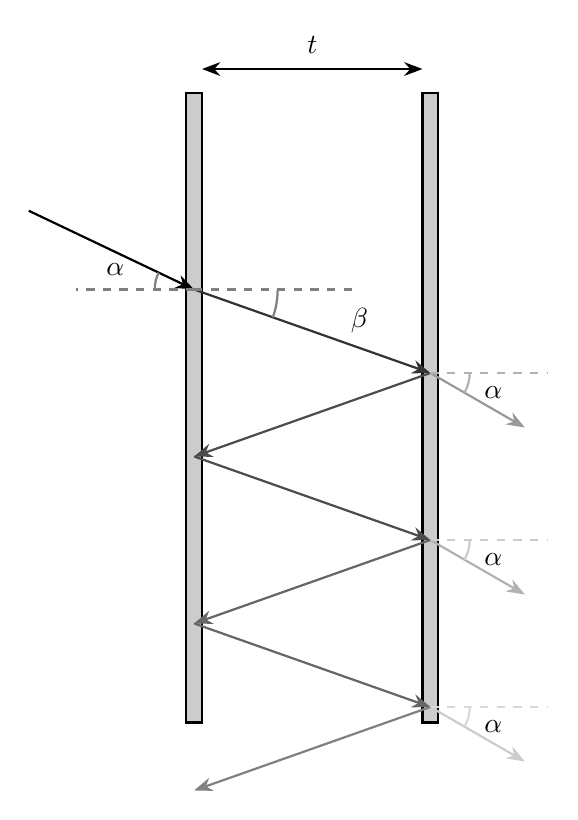
\begin{tikzpicture}[>=Stealth]

% Define parameters
\def\plateheight{8}
\def\platesep{3}
\def\alphaDeg{30}
\def\n{1.5}

% Calculate beta using Snell's law: sin(alpha) = n*sin(beta)
\pgfmathsetmacro{\betaDeg}{asin(sin(\alphaDeg)/\n)}
\pgfmathsetmacro{\dx}{\platesep*tan(\betaDeg)}

% Draw the two parallel plates
\draw[thick, fill=black!20] (0,0) rectangle (0.2,\plateheight);
\draw[thick, fill=black!20] (\platesep,0) rectangle (\platesep+0.2,\plateheight);

% Plate distance label at top
\draw[<->,thick] (0.2,\plateheight+0.3) -- (\platesep,\plateheight+0.3);
\node at (1.6,\plateheight+0.6) {$t$};

% ===== INCOMING RAY =====
\coordinate (start) at (-2, 6.5);
\coordinate (entry) at (0.1, 5.5);

% Draw incident ray
\draw[->,thick,black] (start) -- (entry);

% Normal line (horizontal) for incoming ray
\draw[dashed,thick,black!50] (entry) -- ++(-1.5, 0);

% alpha = angle from horizontal to incoming ray ~ atan2(1.0, 2.1)
\pgfmathsetmacro{\incomingAngle}{atan2(1.0,2.1)}

% Arc from 180 deg (horizontal left) clockwise to incoming ray direction
\draw[thick,black!50] (entry) ++(-0.5,0) arc (180:{180-\incomingAngle}:0.5);
\node at (-0.9, 5.75) {$\alpha$};

% ===== FIRST INTERNAL RAY =====
\coordinate (A1) at (0.1, 5.5);
\coordinate (B1) at (\platesep+0.1, {5.5-\dx});

\draw[->,thick,black!80] (A1) -- (B1);

\draw[dashed,thick,black!50] (A1) -- ++(2.0,0);

\pgfmathsetmacro{\internalAngle}{atan2(-\dx,3.0)}
\pgfmathsetmacro{\arcRadInternal}{1.0/cos(\internalAngle)}

\draw[thick,black!50] (A1) ++(\arcRadInternal,0) arc (0:\internalAngle:\arcRadInternal);
\node at (2.2, 5.10) {$\beta$};

% ===== FIRST TRANSMITTED RAY =====
\coordinate (exit1) at ({\platesep+0.1+1.2}, {5.5-\dx-1.2*tan(\alphaDeg)});
\draw[->,thick,black!40] (B1) -- (exit1);

% ===== FIRST REFLECTION BACK =====
\coordinate (C1) at (0.1, {5.5-2*\dx});
\draw[->,thick,black!70] (B1) -- (C1);

% ===== SECOND INTERNAL RAY =====
\coordinate (D1) at (\platesep+0.1, {5.5-3*\dx});
\draw[->,thick,black!70] (C1) -- (D1);

% ===== SECOND TRANSMITTED RAY =====
\coordinate (exit2) at ({\platesep+0.1+1.2}, {5.5-3*\dx-1.2*tan(\alphaDeg)});
\draw[->,thick,black!30] (D1) -- (exit2);

\draw[dashed,thick,black!20] (D1) -- ++(1.5,0);
\draw[thick,black!20] (D1) ++(0.5,0) arc (0:{-\alphaDeg}:0.5);
\node at ({\platesep+0.9},{5.5-3*\dx-0.25}) {$\alpha$};

% ===== SECOND REFLECTION BACK =====
\coordinate (E1) at (0.1, {5.5-4*\dx});
\draw[->,thick,black!60] (D1) -- (E1);

% ===== THIRD INTERNAL RAY =====
\coordinate (F1) at (\platesep+0.1, {5.5-5*\dx});
\draw[->,thick,black!60] (E1) -- (F1);

% ===== THIRD TRANSMITTED RAY =====
\coordinate (exit3) at ({\platesep+0.1+1.2}, {5.5-5*\dx-1.2*tan(\alphaDeg)});
\draw[->,thick,black!20] (F1) -- (exit3);

\draw[dashed,thick,black!15] (F1) -- ++(1.5,0);
\draw[thick,black!15] (F1) ++(0.5,0) arc (0:{-\alphaDeg}:0.5);
\node at ({\platesep+0.9},{5.5-5*\dx-0.25}) {$\alpha$};

% ===== THIRD REFLECTION BACK =====
\coordinate (G1) at (0.1, {5.5-6*\dx});
\draw[->,thick,black!50] (F1) -- (G1);

\draw[dashed,thick,black!30] (B1) -- ++(1.5,0);
\draw[thick,black!30] (B1) ++(0.5,0) arc (0:{-\alphaDeg}:0.5);
\node at ({\platesep+0.9},{5.5-\dx-0.25}) {$\alpha$};

\end{tikzpicture}
\end{document}
